\حصہ{temporary}
%%%%%%%%%%%%%%%%%%%%%%%%%%%%%%%%%%%%%%%%%
\حصہء{سوالات}
\موٹا{\عددی{x\to \mp \infty} پر حد کا حساب}\\
سوال \حوالہ{سوال_استعمال_ترسیم_تفاعل_الف} تا سوال \حوالہ{سوال_استعمال_ترسیم_تفاعل_ب} میں (ا) \عددی{x\to\infty} پر (ب) \عددی{x\to -\infty} پر حد تلاش کریں۔ (کمپیوٹر پر تفاعل ترسیم کرتے ہوئے حد کی ذہنی تصویر بنانے میں مدد ملتی ہے۔)

\ابتدا{سوال}\شناخت{سوال_استعمال_ترسیم_تفاعل_الف}
$f(x)=\tfrac{2}{x}-3$\\
جواب:\quad
(ا) \عددی{-3}، (ب) \عددی{-3}
\انتہا{سوال}
%=======================
\ابتدا{سوال}
$f(x)=\pi-\tfrac{2}{x^2}$
\انتہا{سوال}
%=============================
\ابتدا{سوال}
$g(x)=\tfrac{1}{2+\tfrac{1}{x}}$\\
جواب:\quad
(ا) \عددی{\tfrac{1}{2}}، (ب) \عددی{\tfrac{1}{2}}
\انتہا{سوال}
%==============
\ابتدا{سوال}
$g(x)=\tfrac{1}{8-\tfrac{5}{x^2}}$
\انتہا{سوال}
%=====================
\ابتدا{سوال}
$h(x)=\tfrac{-5+\tfrac{7}{x}}{3-\tfrac{1}{x^2}}$\\
جواب:\quad
(ا) \عددی{-\tfrac{5}{3}}، (ب) \عددی{-\tfrac{5}{3}}
\انتہا{سوال}
%=================
\ابتدا{سوال}\شناخت{سوال_استعمال_ترسیم_تفاعل_ب}
$h(x)=\tfrac{3-\tfrac{2}{x}}{4+\tfrac{\sqrt{2}}{x^2}}$
\انتہا{سوال}
%===================
سوال \حوالہ{سوال_استعمال_درکار_حد_الف} تا سوال \حوالہ{سوال_استعمال_درکار_حد_ب} میں حد تلاش کریں۔

\ابتدا{سوال}\شناخت{سوال_استعمال_درکار_حد_الف}
$\lim\limits_{x\to\infty}\tfrac{\sin 2x}{x}$\\
جواب:\quad
$0$
\انتہا{سوال}
%=====================
\ابتدا{سوال}
$\lim\limits_{\theta\to\infty}\tfrac{\cos \theta}{3\theta}$
\انتہا{سوال}
%=================
\ابتدا{سوال}
$\lim\limits_{t\to-\infty}\tfrac{2-t+\sin t}{t+\cos t}$\\
جواب:\quad
\عددی{-1}
\انتہا{سوال}
%=========================
\ابتدا{سوال}\شناخت{سوال_استعمال_درکار_حد_ب}
$\lim\limits_{r\to \infty}\tfrac{r+\sin r}{2r+7-5\sin r}$
\انتہا{سوال}
%=========================
\موٹا{ناطق تفاعل کی حد}\\
سوال \حوالہ{سوال_استعمال_ناطق_حد_الف} تا سوال \حوالہ{سوال_استعمال_ناطق_حد_ب} میں دیے ناطق تفاعل کی (ا) \عددی{x\to \infty} اور (ب) \عددی{x\to -\infty} پر حد تلاش کریں۔

\ابتدا{سوال}\شناخت{سوال_استعمال_ناطق_حد_الف}
$f(x)=\tfrac{2x+3}{5x+7}$\\
جواب:\quad
(ا) \عددی{\tfrac{2}{5}}، (ب) \عددی{\tfrac{2}{5}}
\انتہا{سوال}
%======================
\ابتدا{سوال}
$f(x)=\tfrac{2x^3+7}{x^3-x^2+x+7}$
\انتہا{سوال}
%========================
\ابتدا{سوال}
$f(x)=\tfrac{x+1}{x^2+3}$\\
جواب:\quad
(ا) \عددی{0}، (ب) \عددی{0}
\انتہا{سوال}
%=========================
\ابتدا{سوال}
$f(x)=\tfrac{3x+7}{x^2-2}$
\انتہا{سوال}
%=======================
\ابتدا{سوال}
$f(x)=\tfrac{1-12x^3}{4x^2+12}$\\
جواب:\quad
(ا) \عددی{-\infty}، (ب) \عددی{\infty}
\انتہا{سوال}
%=======================
\ابتدا{سوال}
$g(x)=\tfrac{1}{x^3-4x+1}$
\انتہا{سوال}
%========================
\ابتدا{سوال}
$h(x)=\tfrac{7x^3}{x^3-3x^2+6x}$\\
جواب:\quad
(ا) \عددی{7}، (ب) \عددی{7}
\انتہا{سوال}
%=====================
\ابتدا{سوال}
$g(x)=\tfrac{3x^2-6x}{4x-8}$
\انتہا{سوال}
%======================
\ابتدا{سوال}
$f(x)=\tfrac{2x^5+3}{-x^2+x}$\\
جواب:\quad
(ا) \عددی{-\infty}، (ب) \عددی{\infty}
\انتہا{سوال}
%=========================
\ابتدا{سوال}
$g(x)=\tfrac{10x^5+x^4+31}{x^6}$
\انتہا{سوال}
%=======================
\ابتدا{سوال}
$g(x)=\tfrac{x^4}{x^3+1}$\\
جواب:\quad
(ا) \عددی{\infty}، (ب) \عددی{-\infty}
\انتہا{سوال}
%========================
\ابتدا{سوال}
$h(x)=\tfrac{9x^4+x}{2x^4+5x^2-x+6}$
\انتہا{سوال}
%==========================
\ابتدا{سوال}
$h(x)=\tfrac{-2x^3-2x+3}{3x^3+3x^2-5x}$\\
جواب:\quad
(ا) \عددی{-\tfrac{2}{3}}، (ب) \عددی{-\tfrac{2}{3}}
\انتہا{سوال}
%========================
\ابتدا{سوال}\شناخت{سوال_استعمال_ناطق_حد_ب}
$h(x)=\tfrac{-x^4}{x^4-7x^3+7x^2+9}$
\انتہا{سوال}
%=======================

\موٹا{حد برائے غیر عدد صحیح طاقت یا منفی طاقت}\\
ایسی نسبت جس کی نسب نما اور شمار کنندہ میں غیر عدد صحیح یا منفی طاقت پائی جاتی ہوں کی حد بالکل ناطق تفاعل کی حد کی طرح تلاش کی جاتی ہے۔ نسب نما میں \عددی{x} کی بلند تر طاقت سے نسب نما اور شمار کنندہ کو تقسیم کرتے ہوئے آگے بڑھیں۔ سوال \حوالہ{سوال_استعمال_غیر_ناطق_حد_تلاش_الف} تا سوال \حوالہ{سوال_استعمال_غیر_ناطق_حد_تلاش_ب} میں حد تلاش کریں۔

\ابتدا{سوال}\شناخت{سوال_استعمال_غیر_ناطق_حد_تلاش_الف}
$\lim\limits_{x\to\infty}\tfrac{2\sqrt{x}+x^{-1}}{3x-7}$\\
جواب:\quad
\عددی{0}
\انتہا{سوال}
%=========================
\ابتدا{سوال}
$\lim\limits_{x\to\infty}\tfrac{2+\sqrt{x}}{2-\sqrt{x}}$
\انتہا{سوال}
%==========================
\ابتدا{سوال}
$\lim\limits_{x\to -\infty}\tfrac{\sqrt[3]{x}-\sqrt[5]{x}}{\sqrt[3]{x}+\sqrt[5]{x}}$\\
جواب:\quad
\عددی{1}
\انتہا{سوال}
%=============================
\ابتدا{سوال}
$\lim\limits_{x\to\infty}\tfrac{x^{-1}+x^{-4}}{x^{-2}-x^{-3}}$
\انتہا{سوال}
%=====================
\ابتدا{سوال}
$\lim\limits_{x\to\infty}\tfrac{2x^{5/3}-x^{1/3}+7}{x^{8/5}+3x+\sqrt{x}}$\\
جواب:\quad
\عددی{\infty}
\انتہا{سوال}
%===========================
\ابتدا{سوال}\شناخت{سوال_استعمال_غیر_ناطق_حد_تلاش_ب}
$\lim\limits_{x\to-\infty}\tfrac{\sqrt[3]{x}-5x+3}{2x+x^{2/3}-4}$
\انتہا{سوال}
%=========================
\begin{figure}
\centering
\begin{minipage}{0.23\textwidth}
\centering
\begin{tikzpicture}
\begin{axis}[small,width=4cm,axis lines=middle,xlabel={$x$},ylabel={$y$},xlabel style={at={(current axis.right of origin)},anchor=west},
ylabel style={at={(current axis.above origin)},anchor=south},xmin=-3.2,xmax=3.2,ymin=-2.25,ymax=2.5,xtick={-1,1},xticklabels={,$1$},ytick={-2,-1,1,2}]
\draw(axis cs:1,2)node[circ]{}--(axis cs:-1,-2)node[circ]{};
\draw(axis cs:1,2) to [out=-60,in=180](axis cs:3,1);
\draw(axis cs:-1,-2) to [out=120,in=0](axis cs:-3,-1);
\draw(axis cs:0,0)node[circ]{};
\end{axis}
\end{tikzpicture}
\caption{ایک ممکنہ حل برائے سوال \حوالہ{سوال_استعمال_حد_سے_ترسیم_الف}}
\label{شکل_سوال_استعمال_حد_سے_ترسیم_الف}
\end{minipage}\hfill
\begin{minipage}{0.23\textwidth}
\centering
\begin{tikzpicture}
\begin{axis}[small,width=4cm,axis lines=middle,xlabel={$x$},ylabel={$y$},xlabel style={at={(current axis.right of origin)},anchor=west},
ylabel style={at={(current axis.above origin)},anchor=south},xmin=-3.2,xmax=3.2,ymin=-3,ymax=3,xtick={-1,1},ytick={\empty}]
\draw(axis cs:-1,3) to [out=-90,in=180] (axis cs:0,0.5) to [out=0,in=-90] (axis cs:1,3);
\draw(axis cs:-3,-0.01) to [out=0,in=90](axis cs:-1,-3);
\draw(axis cs:1,-3) to [out=90,in=180](axis cs:3,-0.01);
\draw(axis cs:0,0)node[circ]{};
\draw[dashed](axis cs:-1,-3)--(axis cs:-1,3);
\draw[dashed](axis cs:1,-3)--(axis cs:1,3);
\end{axis}
\end{tikzpicture}
\caption{ایک ممکنہ حل برائے سوال \حوالہ{سوال_استعمال_حد_سے_ترسیم_درکار_پ}}
\label{شکل_سوال_استعمال_حد_سے_ترسیم_درکار_پ}
\end{minipage}\hfill
\begin{minipage}{0.23\textwidth}
\centering
\begin{tikzpicture}
\begin{axis}[clip=false,small,width=4cm,axis lines=middle,xlabel={$x$},ylabel={$y$},xlabel style={at={(current axis.right of origin)},anchor=west},
ylabel style={at={(current axis.above origin)},anchor=south},ymin=0]
\addplot[domain=-2:1.5]{1/(x-2)^2};
\addplot[domain=2.5:6]{1/(x-2)^2}node[pos=0.25,right,font=\tiny]{$y=\tfrac{1}{(x-2)^2}$};
\end{axis}
\end{tikzpicture}
\caption{ایک ممکنہ حل برائے سوال \حوالہ{سوال_استعمال_ایجاد_تفاعل_الف}}
\label{شکل_سوال_استعمال_ایجاد_تفاعل_الف}
\end{minipage}\hfill
\begin{minipage}{0.23\textwidth}
\centering
\begin{tikzpicture}
\begin{axis}[clip=false,small,width=4cm,axis lines=middle,xlabel={$x$},ylabel={$y$},xlabel style={at={(current axis.right of origin)},anchor=west},
ylabel style={at={(current axis.above origin)},anchor=south},ymin=-1.25,ymax=1.5,xtick={\empty}]
\addplot[domain=-2:-0.01]{x/(abs(x))};
\addplot[domain=0.01:2]{x/(abs(x))};
\draw(axis cs:-0.5,0.5)node[left,font=\tiny,align=center]{$h(x)=\tfrac{x}{\abs{x}}$\\  $x\ne 0$};
\draw(axis cs:0,-1)node[ocirc]{}  (axis cs:0,1)node[ocirc]{};
\end{axis}
\end{tikzpicture}
\caption{ایک ممکنہ حل برائے سوال \حوالہ{سوال_استعمال_ایجاد_تفاعل_درکار_پ}}
\label{شکل_سوال_استعمال_ایجاد_تفاعل_درکار_پ}
\end{minipage}
\end{figure}
\موٹا{قیمتوں اور حد سے ترسیم کا حصول}\\
سوال \حوالہ{سوال_استعمال_حد_سے_ترسیم_الف} تا سوال \حوالہ{سوال_استعمال_حد_سے_ترسیم_ب} میں دیے شرائط پر پورا اترتی ترسیم کا خاکہ بنائیں۔ ترسیم کا کلیہ درکار نہیں ہے لہٰذا کارتیسی محدد پر ایسی ترسیم کھینچیں جو دیے شرائط پر پورا اترتی ہو۔(ان شرائط کو کئی ترسیمات مطمئن کر سکتی ہیں لہٰذا آپ کے ترسیمات دیے گئے جوابی ترسیمات سے مختلف ہو سکتی ہیں۔)

\ابتدا{سوال}\شناخت{سوال_استعمال_حد_سے_ترسیم_الف}
$f(0)=0,f(1)=2, f(-1)=-2,\lim\limits_{x\to -\infty}=-1,\lim\limits_{x\to\infty}=1$\\
جواب:\quad
شکل \حوالہ{شکل_سوال_استعمال_حد_سے_ترسیم_الف}
\انتہا{سوال}
%=========================
\ابتدا{سوال}
$f(0)=0, \lim\limits_{x\to \mp\infty}f(x)=0,\lim\limits_{x\to 0^+}=2,\lim\limits_{x\to0^-}=-2$
\انتہا{سوال}
%=========================
\ابتدا{سوال}\شناخت{سوال_استعمال_حد_سے_ترسیم_درکار_پ}
$f(0)=0, \lim\limits_{x\to \mp\infty}f(x)=0,\lim\limits_{x\to 1^-}f(x)=\lim\limits_{x\to-1^+}f(x)=\infty,$\\
$\lim\limits_{x\to1^+}f(x)=-\infty, \lim\limits_{x\to-1^-}f(x)=-\infty$\\
جواب:\quad
شکل \حوالہ{شکل_سوال_استعمال_حد_سے_ترسیم_درکار_پ}
\انتہا{سوال}
%=========================
\ابتدا{سوال}\شناخت{سوال_استعمال_حد_سے_ترسیم_ب}
$f(2)=1,f(-1)=0, \lim\limits_{x\to \infty}f(x)=0,\lim\limits_{x\to 0^+}f(x)=\infty,$\\
$\lim\limits_{x\to 0^-}f(x)=-\infty,\lim\limits_{x\to-\infty}f(x)=1$
\انتہا{سوال}
%==========================

\موٹا{تفاعل کی ایجاد}\\
سوال \حوالہ{سوال_استعمال_ایجاد_تفاعل_الف} تا سوال \حوالہ{سوال_استعمال_ایجاد_تفاعل_ب} میں ایسا تفاعل تلاش کریں جو دیے گئے شرائط کو مطمئن کرتا ہو اور اس تفاعل کو ترسیم کریں۔ (چونکہ کئی تفاعل ان شرائط کو مطمئن کر سکتے ہیں لہٰذا آپ کے جوابات دیے گئے جوابات سے مختلف ہو سکتے ہیں۔ آپ ٹکڑوں میں تفاعل کے کلیات استعمال کر سکتے ہیں۔)  

\ابتدا{سوال}\شناخت{سوال_استعمال_ایجاد_تفاعل_الف}
$\lim\limits_{x\to\mp\infty}f(x)=0, \lim\limits_{x\to 2^-}f(x)=\infty,\lim\limits_{x\to 2^+}f(x)=\infty$\\
جواب:\quad
شکل \حوالہ{شکل_سوال_استعمال_ایجاد_تفاعل_الف}
\انتہا{سوال}
%=======================
\ابتدا{سوال}
$\lim\limits_{x\to\mp\infty}g(x)=0, \lim\limits_{x\to 3^-}g(x)=-\infty,\lim\limits_{x\to 3^+}g(x)=\infty$
\انتہا{سوال}
%=======================
\ابتدا{سوال}\شناخت{سوال_استعمال_ایجاد_تفاعل_درکار_پ}
$\lim\limits_{x\to-\infty}h(x)=-1, \lim\limits_{x\to \infty}h(x)=1,\lim\limits_{x\to 0^-}h(x)=-1,\lim\limits_{x\to 0^+}h(x)=1$\\
جواب:\quad
شکل \حوالہ{شکل_سوال_استعمال_ایجاد_تفاعل_درکار_پ}
\انتہا{سوال}
%=======================
\ابتدا{سوال}\شناخت{سوال_استعمال_ایجاد_تفاعل_ب}
$\lim\limits_{x\to\mp\infty}k(x)=1, \lim\limits_{x\to 1^-}k(x)=\infty,\lim\limits_{x\to 1^+}(x)=-\infty$
\انتہا{سوال}
%=======================
\begin{figure}
\centering
\begin{minipage}{0.23\textwidth}
\centering
\begin{tikzpicture}
\begin{axis}[small,width=4cm,axis lines=middle,xlabel={$x$},ylabel={$y$},xlabel style={at={(current axis.right of origin)},anchor=west},
ylabel style={at={(current axis.above origin)},anchor=south},xtick={1}]
\addplot[domain=-2.5:0.9]{1/(x-1)};
\addplot[domain=1.1:4.5]{1/(x-1)}node[pos=0.5,right,font=\tiny]{$y=\tfrac{1}{x-1}$};
\draw[dashed](axis cs:1,-10)--(axis cs:1,10)node[pos=0.2,right,font=\tiny]{$x=1$};
\end{axis}
\end{tikzpicture}
\caption{ترسیم سوال \حوالہ{سوال_استعمال_ناطق_غالب_متقارب_الف}}
\label{شکل_سوال_استعمال_ناطق_غالب_متقارب_الف}
\end{minipage}\hfill
\begin{minipage}{0.23\textwidth}
\centering
\begin{tikzpicture}
\begin{axis}[small,width=4cm,axis lines=middle,xlabel={$x$},ylabel={$y$},xlabel style={at={(current axis.right of origin)},anchor=west},
ylabel style={at={(current axis.above origin)},anchor=south},xtick={-2}]
\addplot[domain=-4.5:-2.1]{1/(2*x+4)};
\addplot[domain=-1.9:2.5]{1/(2*x+4)}node[above left,font=\tiny,xshift=2mm]{$y=\tfrac{1}{2x+4}$};
\draw[dashed](axis cs:-2,-4)--(axis cs:-2,4)node[below left,font=\tiny]{$x=-2$};
\end{axis}
\end{tikzpicture}
\caption{ترسیم سوال \حوالہ{سوال_استعمال_ناطق_غالب_متقارب_درکار_پ}}
\label{شکل_سوال_استعمال_ناطق_غالب_متقارب_درکار_پ}
\end{minipage}\hfill
\begin{minipage}{0.23\textwidth}
\centering
\begin{tikzpicture}
\begin{axis}[clip=false,small,width=4cm,axis lines=middle,xlabel={$x$},ylabel={$y$},xlabel style={at={(current axis.right of origin)},anchor=west},ylabel style={at={(current axis.above origin)},anchor=south},xtick={-2,-3},ytick={1.5}]
\addplot[domain=-4.5:-2.2]{(x+3)/(x+2)};
\addplot[domain=-1.8:1.5]{(x+3)/(x+2)}node[above left,font=\tiny,xshift=2mm]{$y=\tfrac{x+3}{x+2}$};
\draw[dashed](axis cs:-2,-4)--(axis cs:-2,5)node[pos=0.8,left,font=\tiny]{$x=-2$};
\draw[dashed](axis cs:-4.5,1)--(axis cs:1.5,1)node[pos=0.25,above,font=\tiny]{$y=1$};
\addplot[dashed,domain=-4.5:-2.2]{1/(x+2)}node[pos=1,left,font=\tiny]{$y=\tfrac{1}{x+2}$};
\addplot[dashed,domain=-1.8:1.5]{1/(x+2)};
\end{axis}
\end{tikzpicture}
\caption{ترسیم سوال \حوالہ{سوال_استعمال_ناطق_غالب_متقارب_درکار_ت}}
\label{شکل_سوال_استعمال_ناطق_غالب_متقارب_درکار_ت}
\end{minipage}\hfill
\begin{minipage}{0.23\textwidth}
\centering
\begin{tikzpicture}
\begin{axis}[clip=false,small,width=4cm,axis lines=middle,xlabel={$x$},ylabel={$y$},xlabel style={at={(current axis.right of origin)},anchor=west},
ylabel style={at={(current axis.above origin)},anchor=south},xtick={1}]
\addplot[domain=-3.5:0.8]{(2*x^2+x-1)/(x^2-1)};
\addplot[domain=1.2:3.5]{(2*x^2+x-1)/(x^2-1)}node[pos=0.25,right,font=\tiny,xshift=2mm]{$y=\tfrac{2x^2+x-1}{x^2-1}$};
\draw[dashed](axis cs:1,-5)--(axis cs:1,5)node[pos=0.25,right,font=\tiny]{$x=1$};
\draw[dashed](axis cs:-3.5,2)--(axis cs:3.5,2)node[pos=0.25,above,font=\tiny]{$y=2$};
\addplot[dashed,domain=-3.5:0.8]{1/(x-1)}node[pos=0.2,below,font=\tiny]{$y=\tfrac{1}{x-1}$};
\addplot[dashed,domain=1.2:3.5]{1/(x-1)};
\end{axis}
\end{tikzpicture}
\caption{ترسیم سوال \حوالہ{سوال_استعمال_ناطق_غالب_متقارب_درکار_ٹ}}
\label{شکل_سوال_استعمال_ناطق_غالب_متقارب_درکار_ٹ}
\end{minipage}
\end{figure}
%===================================
\begin{figure}
\centering
\begin{minipage}{0.23\textwidth}
\centering
\begin{tikzpicture}
\begin{axis}[clip=false,small,width=4cm,axis lines=middle,xlabel={$x$},ylabel={$y$},xlabel style={at={(current axis.right of origin)},anchor=west},
ylabel style={at={(current axis.above origin)},anchor=south},xtick={-1,1},xticklabels={,$1$},ytick={-1,1}]
\addplot[domain=-3:-0.5]{(x^2-1)/x};
\addplot[domain=0.5:3]{(x^2-1)/x}node[pos=0.6,right,font=\tiny]{$y=\tfrac{x^2-1}{x}$};
\addplot[dashed,domain=-3:3]{x}node[pos=0.8,above left,font=\tiny]{$y=x$};
\addplot[dashed,domain=-3:-0.5]{-1/x}node[left,font=\tiny]{$y=-\tfrac{1}{x}$};
\addplot[dashed,domain=0.5:3]{-1/x};
\end{axis}
\end{tikzpicture}
\caption{ترسیم سوال \حوالہ{سوال_استعمال_ناطق_غالب_متقارب_درکار_ث}}
\label{شکل_سوال_استعمال_ناطق_غالب_متقارب_درکار_ث}
\end{minipage}\hfill
\begin{minipage}{0.23\textwidth}
\centering
\begin{tikzpicture}
\begin{axis}[clip=false,small,width=4cm,axis lines=middle,xlabel={$x$},ylabel={$y$},xlabel style={at={(current axis.right of origin)},anchor=west},
ylabel style={at={(current axis.above origin)},anchor=south},xmin=-2.5,xmax=2.5]
\addplot[domain=-2:-0.5]{(x^4+1)/(x^2)};
\addplot[domain=0.5:2]{(x^4+1)/(x^2)}node[pos=0.5,below right,font=\tiny]{$y=\tfrac{x^4+1}{x^2}$};
\addplot[dashed,domain=-2:2]{x^2}node[pos=0.25,left,font=\tiny]{$y=x^2$};
\addplot[dashed,domain=-2:-0.5]{1/x^2}node[pos=0,above,font=\tiny]{$y=\tfrac{1}{x^2}$};
\addplot[dashed,domain=0.5:2]{1/x^2};
\end{axis}
\end{tikzpicture}
\caption{ترسیم سوال \حوالہ{سوال_استعمال_ناطق_غالب_متقارب_درکار_ج}}
\label{شکل_سوال_استعمال_ناطق_غالب_متقارب_درکار_ج}
\end{minipage}\hfill
\begin{minipage}{0.23\textwidth}
\centering
\begin{tikzpicture}
\begin{axis}[clip=false,small,width=4cm,axis lines=middle,xlabel={$x$},ylabel={$y$},xlabel style={at={(current axis.right of origin)},anchor=west},
ylabel style={at={(current axis.above origin)},anchor=south}]
\addplot[domain=1.1:2]{1/(x^2-1)}node[pos=0.2,right,font=\tiny]{$y=\tfrac{1}{x^2-1}$};
\addplot[domain=-0.9:0.9]{1/(x^2-1)};
\addplot[domain=-1.1:-2]{1/(x^2-1)};
\draw[dashed](axis cs:-1,-5)--(axis cs:-1,5);
\draw[dashed](axis cs:1,-5)--(axis cs:1,5);
\end{axis}
\end{tikzpicture}
\caption{ترسیم سوال \حوالہ{سوال_استعمال_ناطق_غالب_متقارب_درکار_چ}}
\label{شکل_سوال_استعمال_ناطق_غالب_متقارب_درکار_چ}
\end{minipage}\hfill
\begin{minipage}{0.23\textwidth}
\centering
\begin{tikzpicture}
\begin{axis}[clip=false,small,width=4cm,axis lines=middle,xlabel={$x$},ylabel={$y$},xlabel style={at={(current axis.right of origin)},anchor=west},ylabel style={at={(current axis.above origin)},anchor=south},xtick={1},ytick=-1]
\addplot[domain=-3:-1.1]{-(x^2-2)/(x^2-1)};
\addplot[domain=-0.9:0.9]{-(x^2-2)/(x^2-1)};
\addplot[domain=1.1:3]{-(x^2-2)/(x^2-1)}node[pos=0.2,right,font=\tiny]{$y=-\tfrac{x^2-2}{x^2-1}$};
\draw[dashed](axis cs:-1,-5)--(axis cs:-1,5);
\draw[dashed](axis cs:1,-5)--(axis cs:1,5);
\draw[dashed](axis cs:-3,-1)--(axis cs:3,-1);
\addplot[dashed,domain=-3:-1.1]{1/(x^2-1)}node[pos=0.9,left,font=\tiny]{$y=\tfrac{1}{x^2-1}$};
\addplot[dashed,domain=-0.9:0.9]{1/(x^2-1)};
\addplot[dashed,domain=1.1:3]{1/(x^2-1)};
\end{axis}
\end{tikzpicture}
\caption{ترسیم سوال \حوالہ{سوال_استعمال_ناطق_غالب_متقارب_درکار_ح}}
\label{شکل_سوال_استعمال_ناطق_غالب_متقارب_درکار_ح}
\end{minipage}
\end{figure}
%=======================================
\begin{figure}
\centering
\begin{minipage}{0.23\textwidth}
\centering
\begin{tikzpicture}
\begin{axis}[clip=false,small,width=4cm,axis lines=middle,xlabel={$x$},ylabel={$y$},xlabel style={at={(current axis.right of origin)},anchor=west},ylabel style={at={(current axis.above origin)},anchor=south},xtick={1},ytick={4}]
\addplot[domain=-4:0.8]{x^2/(x-1)};
\addplot[domain=1.2:4]{x^2/(x-1)};
\addplot[dashed,domain=-4:4]{x+1}node[pos=0.2,left,font=\tiny]{$y=x+1$};
\addplot[dashed,domain=-4:0.8]{1/(x-1)};
\addplot[dashed,domain=1.2:4]{1/(x-1)}node[pos=0.85,above,font=\tiny]{$y=\tfrac{1}{x-1}$};
\draw(axis cs:-3,3)node[font=\tiny]{$y=\tfrac{x^2}{x-1}$};
\draw[dashed](axis cs:1,-5)--(axis cs:1,6);
\end{axis}
\end{tikzpicture}
\caption{ترسیم سوال \حوالہ{سوال_استعمال_ناطق_غالب_متقارب_درکار_خ}}
\label{شکل_سوال_استعمال_ناطق_غالب_متقارب_درکار_خ}
\end{minipage}\hfill
\begin{minipage}{0.23\textwidth}
\centering
\begin{tikzpicture}
\begin{axis}[clip=false,small,width=4cm,axis lines=middle,xlabel={$x$},ylabel={$y$},xlabel style={at={(current axis.right of origin)},anchor=west},ylabel style={at={(current axis.above origin)},anchor=south},xtick={1,2},ytick={4}]
\addplot[domain=-4:0.6]{(x^2-4)/(x-1)};
\addplot[domain=1.5:4]{(x^2-4)/(x-1)};
\addplot[dashed,domain=-4:4]{x+1}node[pos=0,right,font=\tiny]{$y=x+1$};
\addplot[dashed,domain=-4:0.6]{-3/(x-1)};
\addplot[dashed,domain=1.5:4]{-3/(x-1)}node[pos=0.5,below right,font=\tiny]{$y=-\tfrac{3}{x-1}$};
\draw(axis cs:1,6)node[above right,font=\tiny]{$y=\tfrac{x^2-4}{x-1}$};
\end{axis}
\end{tikzpicture}
\caption{ترسیم سوال \حوالہ{سوال_استعمال_ناطق_غالب_متقارب_درکار_د}}
\label{شکل_سوال_استعمال_ناطق_غالب_متقارب_درکار_د}
\end{minipage}\hfill
\begin{minipage}{0.23\textwidth}
\centering
\begin{tikzpicture}
\begin{axis}[clip=false,small,width=4cm,axis lines=middle,xlabel={$x$},ylabel={$y$},xlabel style={at={(current axis.right of origin)},anchor=west},ylabel style={at={(current axis.above origin)},anchor=south},xtick={1},ytick={3}]
\addplot[domain=-4:0.8]{(x^2-x+1)/(x-1)};
\addplot[domain=1.2:4]{(x^2-x+1)/(x-1)};
\draw(axis cs:0,5)node[left,font=\tiny]{$y=\tfrac{x^2-x+1}{x-1}$};
\addplot[dashed,domain=-4:4]{x}node[pos=0.2,above,font=\tiny]{$y=x$};
\draw[dashed](axis cs:1,-5)--(axis cs:1,5);
\addplot[dashed,domain=-4:0.6]{1/(x-1)};
\addplot[dashed,domain=1.2:4]{1/(x-1)}node[above,font=\tiny]{$y=\tfrac{1}{x-1}$};
\end{axis}
\end{tikzpicture}
\caption{ترسیم  سوال \حوالہ{سوال_استعمال_ناطق_غالب_متقارب_درکار_ڈ}}
\label{شکل_سوال_استعمال_ناطق_غالب_متقارب_درکار_ڈ}
\end{minipage}\hfill
\begin{minipage}{0.23\textwidth}
\centering
\begin{tikzpicture}
\begin{axis}[clip=false,small,width=4cm,axis lines=middle,xlabel={$x$},ylabel={$y$},xlabel style={at={(current axis.right of origin)},anchor=west},ylabel style={at={(current axis.above origin)},anchor=south},xtick={-2,1},ytick={\empty}]
\addplot[domain=-8:-2.6]{(x-1)^3/(x^2+x-2)};
\addplot[domain=-1.6:6]{(x-1)^3/(x^2+x-2)}node[above left,xshift=3mm,font=\tiny]{$y=\tfrac{(x-1)^3}{x^2+x-2}$};
\draw(axis cs:1,0)node[ocirc]{};
\addplot[dashed,domain=-8:6]{x-4}node[pos=0.7,below right,font=\tiny]{$y=x-4$};
\draw[dashed](axis cs:-2,-20)--(axis cs:-2,16);
\addplot[dashed,domain=-8:-2.6]{9/(x+2)}node[pos=0,below,shift={(2mm,1mm)},font=\tiny]{$y=\tfrac{9}{x+2}$};
\addplot[dashed,domain=-1.6:6]{9/(x+2)};
\end{axis}
\end{tikzpicture}
\caption{ترسیم  سوال \حوالہ{سوال_استعمال_ناطق_غالب_متقارب_درکار_ذ}}
\label{شکل_سوال_استعمال_ناطق_غالب_متقارب_درکار_ذ}
\end{minipage}
\end{figure}
%=====================================
\موٹا{ناطق تفاعل کی ترسیم}\\
سوال \حوالہ{سوال_استعمال_ناطق_غالب_متقارب_الف} تا سوال \حوالہ{سوال_استعمال_ناطق_غالب_متقارب_ب} میں دیے گئے ناطق تفاعل ترسیم کریں۔متقارب خطوط اور غالب اجزاء کی ترسیمات بھی شامل کریں۔

\ابتدا{سوال}\شناخت{سوال_استعمال_ناطق_غالب_متقارب_الف}
$y=\tfrac{1}{x-1}$\\
جواب:\quad
شکل \حوالہ{شکل_سوال_استعمال_ناطق_غالب_متقارب_الف}
\انتہا{سوال}
%========================
\ابتدا{سوال}
$y=\tfrac{1}{x+1}$
\انتہا{سوال}
%========================
\ابتدا{سوال}\شناخت{سوال_استعمال_ناطق_غالب_متقارب_درکار_پ}
$y=\tfrac{1}{2x+4}$\\
جواب:\quad
شکل \حوالہ{شکل_سوال_استعمال_ناطق_غالب_متقارب_درکار_پ}
\انتہا{سوال}
%========================
\ابتدا{سوال}
$y=\tfrac{-3}{x-3}$
\انتہا{سوال}
%========================
\ابتدا{سوال}\شناخت{سوال_استعمال_ناطق_غالب_متقارب_درکار_ت}
$y=\tfrac{x+3}{x+2}$\\
جواب:\quad
شکل \حوالہ{شکل_سوال_استعمال_ناطق_غالب_متقارب_درکار_ت}
\انتہا{سوال}
%========================
\ابتدا{سوال}
$y=\tfrac{2x}{x+1}$
\انتہا{سوال}
%========================
\ابتدا{سوال}\شناخت{سوال_استعمال_ناطق_غالب_متقارب_درکار_ٹ}
$y=\tfrac{2x^2+x-1}{x^2-1}$\\
جواب:\quad
شکل \حوالہ{شکل_سوال_استعمال_ناطق_غالب_متقارب_درکار_ٹ}
\انتہا{سوال}
%========================
\ابتدا{سوال}
$y=\tfrac{x^2-49}{x^2+5x-14}$
\انتہا{سوال}
%========================
\ابتدا{سوال}\شناخت{سوال_استعمال_ناطق_غالب_متقارب_درکار_ث}
$y=\tfrac{x^2-1}{x}$\\
جواب:\quad
شکل \حوالہ{شکل_سوال_استعمال_ناطق_غالب_متقارب_درکار_ث}
\انتہا{سوال}
%========================
\ابتدا{سوال}
$y=\tfrac{x^2+4}{2x}$
\انتہا{سوال}
%========================
\ابتدا{سوال}\شناخت{سوال_استعمال_ناطق_غالب_متقارب_درکار_ج}
$y=\tfrac{x^4+1}{x^2}$\\
جواب:\quad
شکل \حوالہ{شکل_سوال_استعمال_ناطق_غالب_متقارب_درکار_ج}
\انتہا{سوال}
%========================
\ابتدا{سوال}
$y=\tfrac{x^3+1}{x^2}$
\انتہا{سوال}
%========================
\ابتدا{سوال}\شناخت{سوال_استعمال_ناطق_غالب_متقارب_درکار_چ}
$y=\tfrac{1}{x^2-1}$\\
جواب:\quad
شکل \حوالہ{شکل_سوال_استعمال_ناطق_غالب_متقارب_درکار_چ}
\انتہا{سوال}
%========================
\ابتدا{سوال}
$y=\tfrac{x^2}{x^2-1}$
\انتہا{سوال}
%========================
\ابتدا{سوال}\شناخت{سوال_استعمال_ناطق_غالب_متقارب_درکار_ح}
$y=-\tfrac{x^2-2}{x^2-1}$\\
جواب:\quad
شکل \حوالہ{شکل_سوال_استعمال_ناطق_غالب_متقارب_درکار_ح}
\انتہا{سوال}
%========================
\ابتدا{سوال}
$y=\tfrac{x^2-4}{x^2-2}$
\انتہا{سوال}
%========================
\ابتدا{سوال}\شناخت{سوال_استعمال_ناطق_غالب_متقارب_درکار_خ}
$y=\tfrac{x^2}{x-1}$\\
جواب:\quad
شکل \حوالہ{شکل_سوال_استعمال_ناطق_غالب_متقارب_درکار_خ}
\انتہا{سوال}
%========================
\ابتدا{سوال}
$y=-\tfrac{x^2}{x+1}$
\انتہا{سوال}
%========================
\ابتدا{سوال}\شناخت{سوال_استعمال_ناطق_غالب_متقارب_درکار_د}
$y=\tfrac{x^2-4}{x-1}$\\
جواب:\quad
شکل \حوالہ{شکل_سوال_استعمال_ناطق_غالب_متقارب_درکار_د}
\انتہا{سوال}
%========================
\ابتدا{سوال}
$y=-\tfrac{x^2-4}{x+1}$
\انتہا{سوال}
%========================
\ابتدا{سوال}\شناخت{سوال_استعمال_ناطق_غالب_متقارب_درکار_ڈ}
$y=\tfrac{x^2-x+1}{x-1}$\\
جواب:\quad
شکل \حوالہ{شکل_سوال_استعمال_ناطق_غالب_متقارب_درکار_ڈ}
\انتہا{سوال}
%========================
\ابتدا{سوال}
$y=-\tfrac{x^2-x+1}{x-1}$
\انتہا{سوال}
%========================
\ابتدا{سوال}\شناخت{سوال_استعمال_ناطق_غالب_متقارب_درکار_ذ}
$y=\tfrac{x^3-3x^2+3x-1}{x^2+x-2}$\\
جواب:\quad
شکل \حوالہ{شکل_سوال_استعمال_ناطق_غالب_متقارب_درکار_ذ}
\انتہا{سوال}
%========================
\ابتدا{سوال}
$y=\tfrac{x^3+x-2}{x-x^2}$
\انتہا{سوال}
%========================
\ابتدا{سوال}
$y=\tfrac{x}{x^2-1}$
\انتہا{سوال}
%========================
\ابتدا{سوال}
$y=\tfrac{x-1}{x^2(x-2)}$
\انتہا{سوال}
%========================
\ابتدا{سوال}
$y=\tfrac{8}{x^2+4}$
\انتہا{سوال}
%========================
\ابتدا{سوال}\شناخت{سوال_استعمال_ناطق_غالب_متقارب_ب}
$y=\tfrac{4x}{x^2+4}$
\انتہا{سوال}
%========================

\موٹا{کمپیوٹر کا استعمال}\\
سوال \حوالہ{سوال_استعمال_کلیہ_ترسیم_الف} تا سوال \حوالہ{سوال_استعمال_کلیہ_ترسیم_ب} کو کمپیوٹر پر ترسیم کریں۔ تفاعل کے کلیہ اور ترسیم کا تعلق سمجھائیں۔

\ابتدا{سوال}\شناخت{سوال_استعمال_کلیہ_ترسیم_الف}
$y=\tfrac{x}{\sqrt{4-x^2}}$
\انتہا{سوال}
%==========================
\ابتدا{سوال}
$y=\tfrac{-1}{\sqrt{4-x^2}}$
\انتہا{سوال}
%==========================
\ابتدا{سوال}
$y=x^{2/3}+\tfrac{1}{x^{1/3}}$
\انتہا{سوال}
%==========================
\ابتدا{سوال}
$y=2\sqrt{x}+\tfrac{2}{\sqrt{x}}-3$
\انتہا{سوال}
%==========================
\ابتدا{سوال}
$y=\sin(\tfrac{\pi}{x^2+1})$
\انتہا{سوال}
%==========================
\ابتدا{سوال}\شناخت{سوال_استعمال_کلیہ_ترسیم_ب}
$y=-\cos(\tfrac{\pi}{x^2+1})$
\انتہا{سوال}
%==========================
\موٹا{اجزاء کی ترسیمات}\\
سوال \حوالہ{سوال_استعمال_اجزاء_سے_پورا_الف} تا سوال \حوالہ{سوال_استعمال_اجزاء_سے_پورا_ب} میں تفاعل کے اجزاء کو انفرادی ایک ساتھ ترسیم کریں۔ان ترسیمات کو دیکھتے ہوئے تفاعل کا خاکہ کھینچیں۔

\ابتدا{سوال}\شناخت{سوال_استعمال_اجزاء_سے_پورا_الف}
$y=\sec x+\tfrac{1}{x},\quad -\tfrac{\pi}{2}<x<\tfrac{\pi}{2}$
\انتہا{سوال}
%=====================
\ابتدا{سوال}
$y=\sec x-\tfrac{1}{x^2},\quad -\tfrac{\pi}{2}<x<\tfrac{\pi}{2}$
\انتہا{سوال}
%=====================
\ابتدا{سوال}
$y=\tan x+\tfrac{1}{x^2},\quad -\tfrac{\pi}{2}<x<\tfrac{\pi}{2}$
\انتہا{سوال}
%=====================
\ابتدا{سوال}\شناخت{سوال_استعمال_اجزاء_سے_پورا_ب}
$y=\tfrac{1}{x}-\tan x,\quad -\tfrac{\pi}{2}<x<\tfrac{\pi}{2}$
\انتہا{سوال}
%=====================
\موٹا{نظریہ اور مثالیں}

\ابتدا{سوال}
\عددی{f(x)=\tfrac{x^3+x^2}{x^2+1}} لیں۔ دکھائیں کہ ایسا \عددی{c} پایا جاتا ہے کہ \عددی{f(c)} کی قیمت درج ذیل ہو۔ 
\begin{multicols}{3}
\begin{enumerate}[a.]
\item
$-2$
\item
$\cos 3$
\item
$\num{5000000}$
\end{enumerate}
\end{multicols}
\انتہا{سوال}
%======================
\ابتدا{سوال}
\عددی{\lim\limits_{x\to\infty}(\sqrt{x^2+x}-\sqrt{x^2-x})} تلاش کریں۔
\انتہا{سوال}
%=================
\ابتدا{سوال}\ترچھا{تشاکلی۔}\quad
فرض کریں وقفہ \عددی{x>0} پر جفت تفاعل بڑھتا ہے۔وقفہ \عددی{x<0} پر تفاعل کا رویہ کیا ہو گا؟
\انتہا{سوال}
%====================
\ابتدا{سوال}\ترچھا{تشاکلی۔}\quad
فرض کریں وقفہ \عددی{x<0} پر جفت تفاعل بڑھتا ہے۔وقفہ \عددی{x>0} پر تفاعل کا رویہ کیا ہو گا؟
\انتہا{سوال}
%====================
\ابتدا{سوال}
فرض کریں \عددی{f(x)} اور \عددی{g(x)} کثیر رکنی ہیں اور \عددی{ \lim_{x\to\infty}\tfrac{f(x)}{g(x)}=2} ہے۔کیا 
\عددی{ \lim_{x\to-\infty}\tfrac{f(x)}{g(x)}} کے بارے میں کچھ اخذ کرنا ممکن ہے؟ اپنے جواب کی وجہ بین کریں۔
\انتہا{سوال}
%======================
\ابتدا{سوال}
فرض کریں \عددی{f(x)} اور \عددی{g(x)} کثیر رکنی ہیں۔ اگر \عددی{g(x)} کبھی بھی صفر نہیں ہو تب کیا \عددی{\tfrac{f(x)}{g(x)}} کی ترسیم کا متقارب ہو گا؟ اپنے جواب کی وجہ پیش کریں۔
\انتہا{سوال}
%======================
\ابتدا{سوال}
دیے گئے ناطق تفاعل کے  کتنے افقی متقارب ہو سکتے ہیں؟ اپنے جواب کی وجہ پیش کریں۔
\انتہا{سوال}
%======================
\ابتدا{سوال}
دیے گئے ناطق تفاعل کے  کتنے انتصابی متقارب ہو سکتے ہیں؟ اپنے جواب کی وجہ پیش کریں۔
\انتہا{سوال}
%======================
\ابتدا{سوال}
\begin{enumerate}[a.]
\item

ایک ترسیم اپنے متقاربی خط کو قطع کر سکتی ہے۔ منحنی \عددی{y=2+\tfrac{\sin x}{x}} (مثال \حوالہ{مثال_استعمال_مسئلہ_بیچ}) متقاربی خط کو لامتناہی بار قطع کرتی ہے۔ دکھائیں کہ \عددی{x\to \infty} پر اس ترسیم کی ڈھلوان متقاربی خط کی ڈھلوان تک پہنچتی ہے۔ 
\item
درج ذیل خواص رکھنے والے تفاعل \عددی{f(x)} کی مثال پیش کریں۔
\begin{enumerate}[1)]
\item
\عددی{x>0} پر \عددی{f} قابل تفرق ہے۔
\item
$\lim\limits_{x\to\infty}f(x)=2$
\item
\عددی{\lim\limits_{x\to\infty}f'(x)} غیر موجود ہے۔
\end{enumerate}
\end{enumerate}
\انتہا{سوال}
%======================
\ابتدا{سوال}
ہم درج ذیل تفاعل کی متقاربی خط تلاش کرنا چاہتے ہیں۔
\begin{align*}
y=\frac{x^2+3x+7}{x+2}
\end{align*}
ایسا کرنے کی خاطر ہم اس تفاعل کو کثیر رکنی اور حاصل تقسیم کا مجموعہ لکھتے ہیں
\begin{align*}
\frac{x^2+3x+7}{x+2}=x+1+\frac{5}{x+2}
\end{align*}
جس کی ترچھی متقارب \عددی{y=x+1} ہے۔

اگر ہم نسب نما اور شمار کنندہ کو \عددی{x} سے تقسیم کریں تب
\begin{align*}
\frac{x^2+3x+7}{x+2}=\frac{x+3+\tfrac{7}{x}}{1+\tfrac{2}{x}}
\end{align*} 
ملتا ہے جس کی متقارب \عددی{y=x+3} ہے۔

ان میں سے کون کا خط متقارب ہے؟ اپنے جواب کی وجہ پیش کریں۔
\انتہا{سوال}
%==========================
سوال \حوالہ{سوال_استعمال_تصدیق_حد_الف} اور سوال \حوالہ{سوال_استعمال_تصدیق_حد_ب} میں حد کی با ضابطہ تعریف استعمال کرتے ہوئے \عددی{x\to \mp\infty} پر دی گئی حد کی تصدیق کریں۔

\ابتدا{سوال}\شناخت{سوال_استعمال_تصدیق_حد_الف}
اگر \عددی{f} کی قیمت مستقل ہو \عددی{f(x)=k} تب \عددی{\lim_{x\to\infty}f(x)=k} ہو گا۔
\انتہا{سوال}
%==============
\ابتدا{سوال}\شناخت{سوال_استعمال_تصدیق_حد_ب}
اگر \عددی{f} کی قیمت مستقل ہو \عددی{f(x)=k} تب \عددی{\lim_{x\to-\infty}f(x)=k} ہو گا۔
\انتہا{سوال}
%===========================
\موٹا{کمپیوٹر ترسیمات کے مزید مشاہدے}\\
سوال \حوالہ{سوال_استعمال_مزید_ترسیم_متقارب_الف} تا سوال \حوالہ{سوال_استعمال_مزید_ترسیم_متقارب_ب} میں تفاعل ترسیم کریں۔ ان تفاعل کے متقاربی خط تلاش کریں۔ متقاربی خط جہاں ہیں، اس کی وجہ پیش کریں۔

\ابتدا{سوال}\شناخت{سوال_استعمال_مزید_ترسیم_متقارب_الف}
$y=-\tfrac{x^2-4}{x+1}$
\انتہا{سوال}
%=======================
\ابتدا{سوال}
$y=\tfrac{x^2+x-6}{2x-2}$
\انتہا{سوال}
%=======================
\ابتدا{سوال}
$y=\tfrac{x^3-x^2-1}{x^2-1}$
\انتہا{سوال}
%=======================
\ابتدا{سوال}\شناخت{سوال_استعمال_مزید_ترسیم_متقارب_ب}
$y=\tfrac{x^3-2x^2+x+1}{x-x^2}$
\انتہا{سوال}
%=======================
سوال \حوالہ{سوال_استعمال_تفاعل_اور_غالب_الف} تا سوال \حوالہ{سوال_استعمال_تفاعل_اور_غالب_ب} میں تفاعل کی ترسیم کے ساتھ غالب اجزاء بھی ترسیم کریں۔تفاعل کی ترسیم اور غالب اجزاء کی ترسیمات کا تعلق بیان کریں۔

\ابتدا{سوال}\شناخت{سوال_استعمال_تفاعل_اور_غالب_الف}
$y=x^3+\tfrac{3}{x}$
\انتہا{سوال}
%==========================
\ابتدا{سوال}
$y=x^3-\tfrac{3}{x}$
\انتہا{سوال}
%==========================
\ابتدا{سوال}
$y=2\sin x+\tfrac{1}{x}$
\انتہا{سوال}
%==========================
\ابتدا{سوال}
$y=2\cos x-\tfrac{1}{x}$
\انتہا{سوال}
%==========================
\ابتدا{سوال}
$y=\tfrac{x^2}{2}+3\sin 2x$
\انتہا{سوال}
%==========================
\ابتدا{سوال}\شناخت{سوال_استعمال_تفاعل_اور_غالب_ب}
$y=(x-1)^{11}+2\sin 2\pi x$
\انتہا{سوال}
%==========================
سوال \حوالہ{سوال_استعمال_ترسیم_سے_رویہ_الف} اور سوال \حوالہ{سوال_استعمال_ترسیم_سے_رویہ_ب} کا تفاعل ترسیم کریں۔اس کے بعد درج ذیل کے جوابات دیں۔
\begin{enumerate}[a.]
\item
\عددی{x\to0^+} اور \عددی{x\to 0^-} پر ترسیم کا رویہ کیسا ہے؟
\item
\عددی{x\to \mp\infty} پر ترسیم کا رویہ کیسا ہے؟
\item
\عددی{x\to 1} اور \عددی{x\to -1} پر ترسیم کا رویہ کیسا ہے؟
\end{enumerate}
اپنے جوابات کی وجہ پیش کریں۔

\ابتدا{سوال}\شناخت{سوال_استعمال_ترسیم_سے_رویہ_الف}
$y=\tfrac{3}{2}(x-\tfrac{1}{x})^{2/3}$
\انتہا{سوال}
%==========================
\ابتدا{سوال}\شناخت{سوال_استعمال_ترسیم_سے_رویہ_ب}
$y=\tfrac{3}{2}(\tfrac{x}{x-1})^{2/3}$
\انتہا{سوال}
%==========================
\ابتدا{سوال}
تفاعل \عددی{y=-\tfrac{x^3-2}{x^2+1}} کو درج ذیل وقفوں پر ترسیم کریں۔
\begin{multicols}{3}
\begin{enumerate}[a.]
\item
$-9\le x\le 9$
\item
$-90\le x\le 90$
\item
$-900\le x\le 900$
\end{enumerate}
\end{multicols}

جزو-1 کی ترسیم بہترین ہو گی۔ جزو-ب میں مبدا کے قریب کچھ ہو گا جو بہتر نظر نہیں آئے گا جبکہ جزو-ج کی ترسیم عین \عددی{y=-x} کی ترسیم نظر آئے گی۔ ایسا کیوں ہے؟
\انتہا{سوال}
%==========================
\ابتدا{سوال}
تفاعل \عددی{y=\tfrac{x^{2/3}}{x^2-1}} کو وقفہ \عددی{-2\le x\le 2} پر ترسیم کریں۔  \عددی{x=-1} اور \عددی{x=1}  کے بیچ ترسیم  نیچے مقعر نظر آئے گی اور مبدا پر کوئی کنگرہ نظر نہیں آئے گا۔مبدا کے بالکل قریب وقفہ پر ترسیم کرتے ہوئے مبدا پر کنگرہ نمودار ہوتا ہے۔ پہلی ترسیم میں کنگرہ کیوں نظر نہیں آیا؟ 
\انتہا{سوال}
%==========================
\موٹا{لامتناہی پر حد واضح کرنا}\\
بعض اوقات متغیرات کی تبدیلی سے ایسا تفاعل حاصل ہوتا ہے جس کی حد  تلاش کرنا ہمیں آتا ہے۔مثال کے طور پر 
\begin{align*}
\lim\limits_{x\to\infty}\sin\tfrac{1}{x}&=\lim\limits_{\theta\to0^+}\sin\theta&& (\theta=\tfrac{1}{x})
\end{align*}
آپ دیکھ سکتے ہیں کہ لامتناہی پر حد کو یوں کمپیوٹر پر دیکھا جا سکتا ہے۔سوال \حوالہ{سوال_استعمال_حد_نظر_آئے_ب} تا سوال \حوالہ{سوال_استعمال_حد_نظر_آئے_الف} میں یوں اس طرح کا طریقہ بیان کریں تا کہ ترسیم پر حد کو دیکھا جا سکے۔ ان حدود کو تلاش کریں۔

\ابتدا{سوال}\شناخت{سوال_استعمال_حد_نظر_آئے_الف}
$\lim\limits_{x\to\mp\infty} x\sin\tfrac{1}{x}$
\انتہا{سوال}
%===========================
\ابتدا{سوال}
$\lim\limits_{x\to-\infty} \tfrac{\cos \tfrac{1}{x}}{1+\tfrac{1}{x}}$
\انتہا{سوال}
%===========================
\ابتدا{سوال}
$\lim\limits_{x\to\mp\infty}\tfrac{3x+4}{2x-5}$
\انتہا{سوال}
%===========================
\ابتدا{سوال}
$\lim\limits_{x\to\infty} (\tfrac{1}{x})^{1/x}$
\انتہا{سوال}
%===========================
\ابتدا{سوال}
$\lim\limits_{x\to\mp\infty} (3+\tfrac{2}{x})(\cos \tfrac{1}{x})$
\انتہا{سوال}
%===========================
\ابتدا{سوال}\شناخت{سوال_استعمال_حد_نظر_آئے_ب}
$\lim\limits_{x\to\infty} (\tfrac{3}{x^2}-\cos\tfrac{1}{x})(1+\sin\tfrac{1}{x})$
\انتہا{سوال}
%===========================
